The main ingredients of a training phase are:
\begin{itemize}
\item The Model: the neural network that contains weight and parameters
\item The dataset: it is the source where extract information and knowledge
\item Loss function: the function that tells the model what is learning
\item Optimizer: the technique used to update the weights
\end{itemize}
When u want to train a model u can use different approaches:
\begin{itemize}
\item Supervised Learning: when you have labeled data
\item Unsupervised Learning when your data are not labeled
\item Reinforcement Learning: when your model try to learn through experience and not data
\end{itemize}
But for each kind of learning you have to set up a function that tell to the model how to improve him self. This function is called \textbf{Objective Function, Loss Function, Target Function etc etc} and it is fundamental for:
\begin{itemize}
\item Tell the model how to update weights in order to get better result
\item Control the training of the model
\item Add extra information to the model
\item Avoid bad outcome (Overfitting, not-convergence)
\end{itemize}

\section{Objective function: overview}

\section{Different kinds of Loss Function}

\section{Optimizer}
Let's say we have a very easy model that we can represent using the equation:
\begin{equation}
M(\textbf{x}) = Tanh(\textbf{x}\textbf{W} + \textbf{b})
\end{equation}
Let's say the input is a vector of 2 dimension $(x_0, x_1)$ and the output is a 2 dims vector $(o_0, o_1)$. So the matrix of weights $\textbf{W}$ is a 2x2 matrix.
Let's define a loss function like the MSE = $\frac{\sum_{i=0}^2 (t_i - o_i)^2}{2}$

Now we have our sample $(x_n, t_n) = ([1,1], [0,0])$ and the model generates $[1,-1]$ so we compute the MSE = 1. We want our model itself and reduce the loss but how. In this case in order to reduce the loss we would need to reduce the difference between our model prediction and target $0 - 1, 0 - (-1)$. So we would need to reduce the first value and raise the second. The first value is obtained through the equation:
\begin{equation}
Tanh(\textbf{x}*\textbf{w}_{c1} + b)
\end{equation}
where $\textbf{w}_{c1}$ is the first column of $W$ and $b$ is the first value of the bias vector.
In the same way we know the second value is obtained using the equation:
\begin{equation}
Tanh(\textbf{x}*\textbf{w}_{c2} + b)
\end{equation}
So in order to minimize the loss function we need to reduce $\textbf{w}_{c1}$ and raise $\textbf{w}_{c2}$.

\subsection{BackPropagation and lr}

\begin{figure}
    \centering
    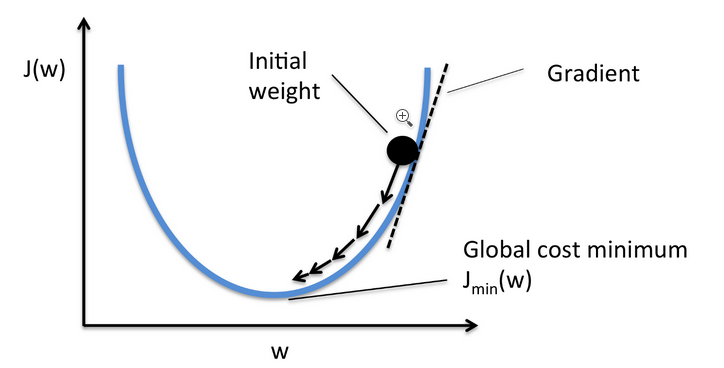
\includegraphics[scale=0.65]{img/gradient.png}
    \caption{How the backpropagation works}
    \label{img:gradient}
\end{figure}

So the idea is we needs to adjust each parameters in a model in order to minimize the loss. In order to automatize this process we need a technique that determines for each parameter if it needs to be raised or lowered. This technique is called \textbf{Back Propagation of the Gradient}. The idea is: the derivative of a function respect a variable tells us if moving forward or backward that variable the output of the function will raise or decrease.  The is exactly what we need. 

Let's define the \textbf{Gradient} as the vectors that contains the partial derivative of each parameters respect the loss function. If the partial derivative is positive so we know that, in order to lower the loss, we need to reduce the value of that parameter otherwise we need to raise the value of that parameter. Geometrically the gradient is the vector that points to the direction where function raise most. 
So the update step is doing by:
\begin{equation}
w_i^t = w_i^{t-1} + \alpha\bigtriangledown_{wi} 
\end{equation}
where $w_i^t$ is the weight $i$ at the time $t$, $\bigtriangledown_{wi} $ is the gradient of the function, in this case it represent the partial derivative of the loss function respect the parameter $wi$. The $\alpha$ represent how much the weight will be incresed or decreased. This value is called \textbf{Learning Rate}



So this is the overview on how weight are update but what is an Optimizer?
The optimizer is the selected technique to update weight, the Back propagation of the Gradient is a technique but also the basic technique, the others will extend this concept in order to make the process faster.

\subsection{}
